\documentclass[]{article}
\usepackage{lmodern}
\usepackage{amssymb,amsmath}
\usepackage{ifxetex,ifluatex}
\usepackage{fixltx2e} % provides \textsubscript
\ifnum 0\ifxetex 1\fi\ifluatex 1\fi=0 % if pdftex
  \usepackage[T1]{fontenc}
  \usepackage[utf8]{inputenc}
\else % if luatex or xelatex
  \ifxetex
    \usepackage{mathspec}
  \else
    \usepackage{fontspec}
  \fi
  \defaultfontfeatures{Ligatures=TeX,Scale=MatchLowercase}
\fi
% use upquote if available, for straight quotes in verbatim environments
\IfFileExists{upquote.sty}{\usepackage{upquote}}{}
% use microtype if available
\IfFileExists{microtype.sty}{%
\usepackage{microtype}
\UseMicrotypeSet[protrusion]{basicmath} % disable protrusion for tt fonts
}{}
\usepackage[margin=1in]{geometry}
\usepackage{hyperref}
\hypersetup{unicode=true,
            pdfborder={0 0 0},
            breaklinks=true}
\urlstyle{same}  % don't use monospace font for urls
\usepackage{color}
\usepackage{fancyvrb}
\newcommand{\VerbBar}{|}
\newcommand{\VERB}{\Verb[commandchars=\\\{\}]}
\DefineVerbatimEnvironment{Highlighting}{Verbatim}{commandchars=\\\{\}}
% Add ',fontsize=\small' for more characters per line
\usepackage{framed}
\definecolor{shadecolor}{RGB}{248,248,248}
\newenvironment{Shaded}{\begin{snugshade}}{\end{snugshade}}
\newcommand{\KeywordTok}[1]{\textcolor[rgb]{0.13,0.29,0.53}{\textbf{#1}}}
\newcommand{\DataTypeTok}[1]{\textcolor[rgb]{0.13,0.29,0.53}{#1}}
\newcommand{\DecValTok}[1]{\textcolor[rgb]{0.00,0.00,0.81}{#1}}
\newcommand{\BaseNTok}[1]{\textcolor[rgb]{0.00,0.00,0.81}{#1}}
\newcommand{\FloatTok}[1]{\textcolor[rgb]{0.00,0.00,0.81}{#1}}
\newcommand{\ConstantTok}[1]{\textcolor[rgb]{0.00,0.00,0.00}{#1}}
\newcommand{\CharTok}[1]{\textcolor[rgb]{0.31,0.60,0.02}{#1}}
\newcommand{\SpecialCharTok}[1]{\textcolor[rgb]{0.00,0.00,0.00}{#1}}
\newcommand{\StringTok}[1]{\textcolor[rgb]{0.31,0.60,0.02}{#1}}
\newcommand{\VerbatimStringTok}[1]{\textcolor[rgb]{0.31,0.60,0.02}{#1}}
\newcommand{\SpecialStringTok}[1]{\textcolor[rgb]{0.31,0.60,0.02}{#1}}
\newcommand{\ImportTok}[1]{#1}
\newcommand{\CommentTok}[1]{\textcolor[rgb]{0.56,0.35,0.01}{\textit{#1}}}
\newcommand{\DocumentationTok}[1]{\textcolor[rgb]{0.56,0.35,0.01}{\textbf{\textit{#1}}}}
\newcommand{\AnnotationTok}[1]{\textcolor[rgb]{0.56,0.35,0.01}{\textbf{\textit{#1}}}}
\newcommand{\CommentVarTok}[1]{\textcolor[rgb]{0.56,0.35,0.01}{\textbf{\textit{#1}}}}
\newcommand{\OtherTok}[1]{\textcolor[rgb]{0.56,0.35,0.01}{#1}}
\newcommand{\FunctionTok}[1]{\textcolor[rgb]{0.00,0.00,0.00}{#1}}
\newcommand{\VariableTok}[1]{\textcolor[rgb]{0.00,0.00,0.00}{#1}}
\newcommand{\ControlFlowTok}[1]{\textcolor[rgb]{0.13,0.29,0.53}{\textbf{#1}}}
\newcommand{\OperatorTok}[1]{\textcolor[rgb]{0.81,0.36,0.00}{\textbf{#1}}}
\newcommand{\BuiltInTok}[1]{#1}
\newcommand{\ExtensionTok}[1]{#1}
\newcommand{\PreprocessorTok}[1]{\textcolor[rgb]{0.56,0.35,0.01}{\textit{#1}}}
\newcommand{\AttributeTok}[1]{\textcolor[rgb]{0.77,0.63,0.00}{#1}}
\newcommand{\RegionMarkerTok}[1]{#1}
\newcommand{\InformationTok}[1]{\textcolor[rgb]{0.56,0.35,0.01}{\textbf{\textit{#1}}}}
\newcommand{\WarningTok}[1]{\textcolor[rgb]{0.56,0.35,0.01}{\textbf{\textit{#1}}}}
\newcommand{\AlertTok}[1]{\textcolor[rgb]{0.94,0.16,0.16}{#1}}
\newcommand{\ErrorTok}[1]{\textcolor[rgb]{0.64,0.00,0.00}{\textbf{#1}}}
\newcommand{\NormalTok}[1]{#1}
\usepackage{graphicx,grffile}
\makeatletter
\def\maxwidth{\ifdim\Gin@nat@width>\linewidth\linewidth\else\Gin@nat@width\fi}
\def\maxheight{\ifdim\Gin@nat@height>\textheight\textheight\else\Gin@nat@height\fi}
\makeatother
% Scale images if necessary, so that they will not overflow the page
% margins by default, and it is still possible to overwrite the defaults
% using explicit options in \includegraphics[width, height, ...]{}
\setkeys{Gin}{width=\maxwidth,height=\maxheight,keepaspectratio}
\IfFileExists{parskip.sty}{%
\usepackage{parskip}
}{% else
\setlength{\parindent}{0pt}
\setlength{\parskip}{6pt plus 2pt minus 1pt}
}
\setlength{\emergencystretch}{3em}  % prevent overfull lines
\providecommand{\tightlist}{%
  \setlength{\itemsep}{0pt}\setlength{\parskip}{0pt}}
\setcounter{secnumdepth}{0}
% Redefines (sub)paragraphs to behave more like sections
\ifx\paragraph\undefined\else
\let\oldparagraph\paragraph
\renewcommand{\paragraph}[1]{\oldparagraph{#1}\mbox{}}
\fi
\ifx\subparagraph\undefined\else
\let\oldsubparagraph\subparagraph
\renewcommand{\subparagraph}[1]{\oldsubparagraph{#1}\mbox{}}
\fi

%%% Use protect on footnotes to avoid problems with footnotes in titles
\let\rmarkdownfootnote\footnote%
\def\footnote{\protect\rmarkdownfootnote}

%%% Change title format to be more compact
\usepackage{titling}

% Create subtitle command for use in maketitle
\newcommand{\subtitle}[1]{
  \posttitle{
    \begin{center}\large#1\end{center}
    }
}

\setlength{\droptitle}{-2em}
  \title{}
  \pretitle{\vspace{\droptitle}}
  \posttitle{}
  \author{}
  \preauthor{}\postauthor{}
  \date{}
  \predate{}\postdate{}

\geometry{ %--- Removed margins on top and bottom for BB posts
        top=4mm,
        bottom=3mm,
}
\usepackage[T1]{fontenc} % Use 8-bit encoding that has 256 glyphs
\usepackage{fourier} % Use the Adobe Utopia font 
\usepackage[english]{babel} % English language/hyphenation
\usepackage{amsmath,amsfonts,amsthm} % Math packages
\usepackage{hanging}
\usepackage{sectsty} % Allows customizing section commands
\usepackage{natbib}
\usepackage{parskip}
\usepackage{color}
\usepackage{easylist}
\usepackage{setspace}
\usepackage[table]{xcolor}
\renewcommand{\&}{and}
\bibliographystyle{apalike2}

\begin{document}

\newcommand{\horrule}[1]{\rule{\linewidth}{#1}}

\title{
        \normalfont \normalsize
        \horrule{0.5pt} \\[0.4cm]
        \large Prostate Cancer Prediction  \\ 
        \horrule{2pt} \\[0.5cm]
}

\author{Gary Seamans}\date{\normalsize\today}\maketitle

\pagenumbering{gobble}

\begin{itemize}
\tightlist
\item
  This example predicts tumor spread in this dataset of 97 men who had
  undergone a biopsy.
\item
  The measures to be used for prediction are BPH, PSA, Gleason Score,
  CP, and size of prostate.
\end{itemize}

Tumor spread is indicated by the presence of cancer outside of the
prostrate. In this dataset that is indicated by capsular penetration
(lcp).

\section{Data Preparation}\label{data-preparation}

The initial step was to load the Prostate Cancer dataset, examine the
data, and determine if any adjustments will be necessary.

\subsection{Load the data}\label{load-the-data}

\begin{Shaded}
\begin{Highlighting}[]
\KeywordTok{library}\NormalTok{(}\StringTok{'lasso2'}\NormalTok{)}
\KeywordTok{data}\NormalTok{(}\StringTok{'Prostate'}\NormalTok{)}
\end{Highlighting}
\end{Shaded}

\subsection{Examine the data}\label{examine-the-data}

First a table of the definitions of the \emph{datadefinitions.csv}.

\begin{Shaded}
\begin{Highlighting}[]
\NormalTok{## Load the data}
\NormalTok{definitions <-}\StringTok{ }\KeywordTok{read.csv}\NormalTok{(}\DataTypeTok{file =} \StringTok{"datadefinitions.csv"}\NormalTok{)}
\NormalTok{## Load the xtable library for LaTex tables}
\KeywordTok{library}\NormalTok{(xtable)}

\NormalTok{## Source the code to create pretty str() tables}
\KeywordTok{source}\NormalTok{(}\StringTok{'strtable.R'}\NormalTok{)}

\NormalTok{## Remove all but the assignment variables from the dataset}
\NormalTok{prostateSubset <-}\StringTok{ }\NormalTok{Prostate[}\KeywordTok{c}\NormalTok{(}\DecValTok{2}\NormalTok{,}\DecValTok{4}\NormalTok{,}\DecValTok{6}\NormalTok{,}\DecValTok{7}\NormalTok{,}\DecValTok{9}\NormalTok{)]}
\KeywordTok{print}\NormalTok{(}\KeywordTok{xtable}\NormalTok{(}\KeywordTok{strtable}\NormalTok{(prostateSubset), }\DataTypeTok{caption =} \StringTok{"Data Types"}\NormalTok{))}
\KeywordTok{print}\NormalTok{(}\KeywordTok{xtable}\NormalTok{(definitions, }\DataTypeTok{caption =} \StringTok{"Data Descriptions"}\NormalTok{), }
      \DataTypeTok{include.rownames =} \OtherTok{FALSE}\NormalTok{)}
\end{Highlighting}
\end{Shaded}

\begin{table}[htb]
\centering
\caption{Data Descriptions} 
\vspace{0.2cm}
\begin{tabular}{ll}
  \hline
Name & Description \\ 
  \hline
lcavol &  log(cancer volume) \\ 
  * lweight &  log(prostate weight) \\ 
  age &  age \\ 
  * lbph &  log(benign prostatic hyperplasia amount) \\ 
  svi &  seminal vesicle invasion \\ 
  * lcp, log(capsular penetration) \\
  * gleason &  Gleason score \\ 
  pgg45 &  percentage Gleason scores 4 or 5 \\ 
  * lpsa &  log(prostate specific antigen) \\ 
   \hline
\end{tabular}
\end{table}

The datatypes for the variables that will be used in creating the
decision tree are shown in table 2. The dependent variable is
highlighted in red. Only those variables that will be used in the
analysis are shown in table 2.

\begin{table}[htb]
\centering
\caption{Data Types} 
\vspace{0.2cm}
\begin{tabular}{rllll}
  \hline
 & variable & class & levels & examples \\ 
  \hline
   2 & lweight & numeric &  & 2.769 3.319, 2.691 ... \\ 
   4 & lbph & numeric &  & -1.386, -1.386, -1.386 ... \\ 
  \rowcolor{red!30} 6 & lcp & numeric &  & -1.386 -1.386, -1.386, ... \\ 
   7 & gleason & numeric &  & 6, 6, 7, 6, ... \\ 
   9 & lpsa & numeric &  & -0.430, -0.162, -0.162 ... \\ 
   \hline
\end{tabular}
\end{table}

Lets print a summary of the data to get a better idea of how our
variables are distributed.

\begin{Shaded}
\begin{Highlighting}[]
\NormalTok{## Print a summary of the data}
\KeywordTok{print}\NormalTok{(}\KeywordTok{xtable}\NormalTok{(}\KeywordTok{summary}\NormalTok{(prostateSubset), }\DataTypeTok{caption =} \StringTok{"Prostate Subset Summary"}\NormalTok{), }
      \DataTypeTok{include.rownames =} \OtherTok{FALSE}\NormalTok{)}
\end{Highlighting}
\end{Shaded}

\begin{table}[htb]
\centering
\caption{Prostate Subset Summary} 
\vspace{0.2cm}
\begin{tabular}{lllll}
  \hline
   lweight &      lbph &      lcp &    gleason &      lpsa \\ 
  \hline
Min.   :2.375   & Min.   :-1.3863   & Min.   :-1.3863   & Min.   :6.000   & Min.   :-0.4308   \\ 
  1st Qu.:3.376   & 1st Qu.:-1.3863   & 1st Qu.:-1.3863   & 1st Qu.:6.000   & 1st Qu.: 1.7317   \\ 
  Median :3.623   & Median : 0.3001   & Median :-0.7985   & Median :7.000   & Median : 2.5915   \\ 
  Mean   :3.653   & Mean   : 0.1004   & Mean   :-0.1794   & Mean   :6.753   & Mean   : 2.4784   \\ 
  3rd Qu.:3.878   & 3rd Qu.: 1.5581   & 3rd Qu.: 1.1787   & 3rd Qu.:7.000   & 3rd Qu.: 3.0564   \\ 
  Max.   :6.108   & Max.   : 2.3263   & Max.   : 2.9042   & Max.   :9.000   & Max.   : 5.5829   \\ 
   \hline
\end{tabular}
\end{table}

\section{Create a decision tree}\label{create-a-decision-tree}

To create a decision tree for predicting whether or not the cancer has
spread outside the prostate (lcp) the following \emph{R} code was used:

\begin{Shaded}
\begin{Highlighting}[]
\KeywordTok{library}\NormalTok{(rpart)}
\KeywordTok{library}\NormalTok{(rpart.plot)}
\NormalTok{## Now create/grow the tree}
\NormalTok{## Since lcp is continuous ranging from -1.3863 to 2.9042 }
\NormalTok{## we'll use a control point of 0.0}
\NormalTok{dt <-}\StringTok{ }\KeywordTok{rpart}\NormalTok{(lcp }\OperatorTok{~}\StringTok{ }\NormalTok{lweight }\OperatorTok{+}\StringTok{ }\NormalTok{lbph }\OperatorTok{+}\StringTok{ }\NormalTok{gleason }\OperatorTok{+}\StringTok{ }\NormalTok{lpsa, }\DataTypeTok{data =}\NormalTok{ prostateSubset, }
            \DataTypeTok{control =} \KeywordTok{rpart.control}\NormalTok{(}\DataTypeTok{cp =} \FloatTok{0.0}\NormalTok{))}
\NormalTok{## Now print the decision tree}
\NormalTok{rpart.plot}\OperatorTok{::}\KeywordTok{rpart.plot}\NormalTok{(dt, }\DataTypeTok{type =} \DecValTok{4}\NormalTok{)}
\end{Highlighting}
\end{Shaded}

\begin{figure}[htp]
\caption{Decision Tree}
\scalebox{0.9}{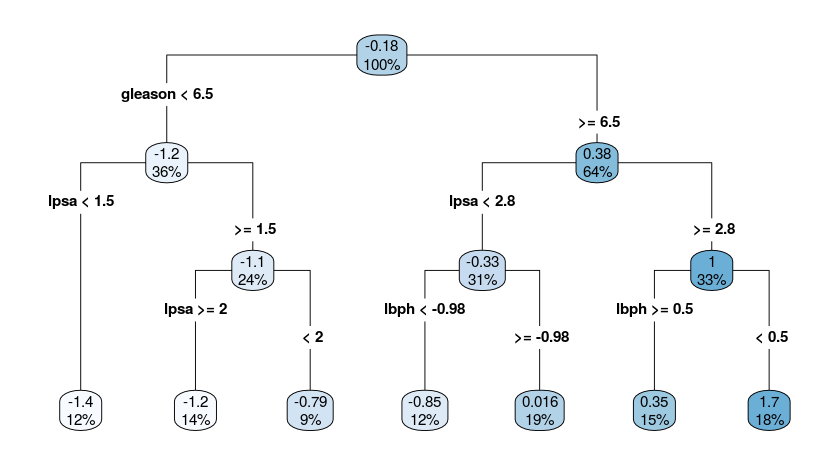
\includegraphics{DecisionTree.png}}
\end{figure}

\begin{shaded}
\begin{verbatim}
Call:
rpart(formula = lcp ~ lweight + lbph + gleason + lpsa, data = prostateSubset, 
    control = rpart.control(cp = 0))
  n= 97 

           CP nsplit rel error    xerror      xstd
1 0.287761884      0 1.0000000 1.0100242 0.1049737
2 0.157270357      1 0.7122381 0.9311028 0.1171615
3 0.074627049      2 0.5549678 0.7996757 0.1158883
4 0.028844280      3 0.4803407 0.7021377 0.1053865
5 0.005079222      4 0.4514964 0.6759693 0.1043335
6 0.000000000      6 0.4413380 0.6730510 0.1029787

Variable importance
   lpsa gleason    lbph lweight 
     41      36      14      10 

Node number 1: 97 observations,    complexity param=0.2877619
  mean=-0.1793656, MSE=1.934946 
  left son=2 (35 obs) right son=3 (62 obs)
  Primary splits:
      gleason < 6.5        to the left,  improve=0.28776190, (0 missing)
      lpsa    < 2.847795   to the left,  improve=0.27998210, (0 missing)
      lweight < 3.355056   to the left,  improve=0.05829831, (0 missing)
      lbph    < 2.040693   to the right, improve=0.02812798, (0 missing)
  Surrogate splits:
      lpsa < 2.066682   to the left,  agree=0.794, adj=0.429, (0 split)

Node number 2: 35 observations,    complexity param=0.005079222
  mean=-1.172511, MSE=0.3564017 
  left son=4 (12 obs) right son=5 (23 obs)
  Primary splits:
      lpsa    < 1.469912   to the left,  improve=0.06690534, (0 missing)
      lweight < 3.347753   to the left,  improve=0.03306504, (0 missing)
      lbph    < -1.092401  to the right, improve=0.01534593, (0 missing)
  Surrogate splits:
      lweight < 3.613572   to the left,  agree=0.714, adj=0.167, (0 split)

Node number 3: 62 observations,    complexity param=0.1572704
  mean=0.3812811, MSE=1.954932 
  left son=6 (30 obs) right son=7 (32 obs)
  Primary splits:
      lpsa    < 2.833001   to the left,  improve=0.24353660, (0 missing)
      lweight < 3.189355   to the left,  improve=0.08617635, (0 missing)
      lbph    < 1.94384    to the right, improve=0.03940827, (0 missing)
  Surrogate splits:
      lweight < 3.517497   to the left,  agree=0.645, adj=0.267, (0 split)
      lbph    < -0.5537256 to the left,  agree=0.532, adj=0.033, (0 split)

Node number 4: 12 observations
  mean=-1.386294, MSE=0 

Node number 5: 23 observations,    complexity param=0.005079222
  mean=-1.060972, MSE=0.5060643 
  left son=10 (14 obs) right son=11 (9 obs)
  Primary splits:
      lpsa    < 1.966231   to the right, improve=0.09210508, (0 missing)
      lbph    < -1.092401  to the right, improve=0.06691219, (0 missing)
      lweight < 3.65838    to the right, improve=0.06200897, (0 missing)
  Surrogate splits:
      lweight < 3.458693   to the right, agree=0.696, adj=0.222, (0 split)

Node number 6: 30 observations,    complexity param=0.02884428
  mean=-0.3313459, MSE=1.433503 
  left son=12 (12 obs) right son=13 (18 obs)
  Primary splits:
      lbph    < -0.9830564 to the left,  improve=0.12588690, (0 missing)
      lweight < 3.401163   to the left,  improve=0.06387888, (0 missing)
      lpsa    < 2.612773   to the right, improve=0.02068067, (0 missing)
  Surrogate splits:
      lweight < 3.005655   to the left,  agree=0.733, adj=0.333, (0 split)
      lpsa    < 1.434446   to the left,  agree=0.733, adj=0.333, (0 split)

Node number 7: 32 observations,    complexity param=0.07462705
  mean=1.049369, MSE=1.521332 
  left son=14 (15 obs) right son=15 (17 obs)
  Primary splits:
      lbph    < 0.4989354  to the right, improve=0.28771530, (0 missing)
      lpsa    < 3.523388   to the left,  improve=0.08441155, (0 missing)
      lweight < 3.63538    to the right, improve=0.04055550, (0 missing)
  Surrogate splits:
      lweight < 3.63538    to the right, agree=0.688, adj=0.333, (0 split)
      lpsa    < 2.993028   to the left,  agree=0.688, adj=0.333, (0 split)

Node number 10: 14 observations
  mean=-1.234074, MSE=0.09139957 

Node number 11: 9 observations
  mean=-0.7917025, MSE=1.031981 

Node number 12: 12 observations
  mean=-0.8516236, MSE=0.5698761 

Node number 13: 18 observations
  mean=0.01550589, MSE=1.708489 

Node number 14: 15 observations
  mean=0.3450452, MSE=1.462536 

Node number 15: 17 observations
  mean=1.670831, MSE=0.7492848 
\end{verbatim}
\end{shaded}

Note that \emph{lweight} is the least important predictive variable and
was not shown in the graphic.

Next I'll validate the model and see if we should do some pruning.

\begin{Shaded}
\begin{Highlighting}[]
\KeywordTok{print}\NormalTok{(}\KeywordTok{xtable}\NormalTok{(}\KeywordTok{printcp}\NormalTok{(dt)),}\DataTypeTok{include.rownames =} \OtherTok{FALSE}\NormalTok{)}
\end{Highlighting}
\end{Shaded}

\begin{table}[htb]
\centering
\caption{ printcp()}
\vspace{0.2cm}
\begin{tabular}{rrrrr}
  \hline
CP & nsplit & rel error & xerror & xstd \\ 
  \hline
0.29 & 0.00 & 1.00 & 1.01 & 0.10 \\ 
  0.16 & 1.00 & 0.71 & 0.93 & 0.12 \\ 
  0.07 & 2.00 & 0.55 & 0.80 & 0.12 \\ 
  0.03 & 3.00 & 0.48 & 0.70 & 0.11 \\ 
  0.01 & 4.00 & 0.45 & 0.68 & 0.10 \\ 
  0.00 & 6.00 & 0.44 & 0.67 & 0.10 \\ 
   \hline
\end{tabular}
\end{table}

Now I should use the CP which generates the least \emph{xerror}. It is
easy to see that the \textbf{CP} value to use is \emph{0.0}, lucky guess
on my part.

If the \textbf{CP} table is very large I could use the below to find the
value of \textbf{CP} to use to prune the tree.

\begin{Shaded}
\begin{Highlighting}[]
\NormalTok{dt}\OperatorTok{$}\NormalTok{cptable[}\KeywordTok{which.min}\NormalTok{(dt}\OperatorTok{$}\NormalTok{cptable[,}\StringTok{"xerror"}\NormalTok{]),}\StringTok{"CP"}\NormalTok{]}
\NormalTok{[}\DecValTok{1}\NormalTok{] }\DecValTok{0}
\end{Highlighting}
\end{Shaded}

Which returns the same value that we found by visually examining the
\textbf{CP} table and the value that was originally used, so no further
pruning is required. I can also plot the \textbf{CP} table to visualize
the deviation until the minimum error is calculated.

\begin{Shaded}
\begin{Highlighting}[]
\KeywordTok{plotcp}\NormalTok{(dt, }\DataTypeTok{col =} \StringTok{"red"}\NormalTok{)}
\end{Highlighting}
\end{Shaded}

\begin{figure}[htb]
\caption{Plot Cutoff Point}
\vspace{0.2cm}
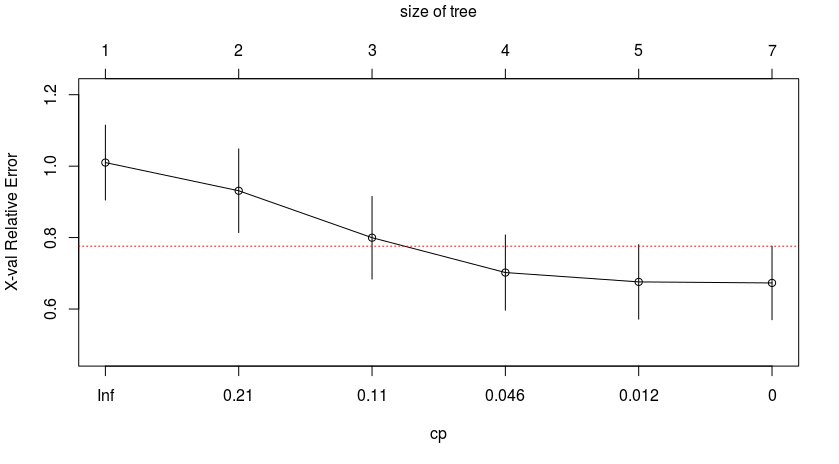
\includegraphics{plotcp.png}
\end{figure}

\subsection{Just for fun}\label{just-for-fun}

Since we're really not concerned with \emph{how invasive} the cancer is,
just that it has spread outside of the prostate, I'll change the
\emph{lcp} variable to a factor and redo the calculations. We are trying
to predict the probability of whether or not the cancer has spread
outside the prostate indicated by an \emph{lcp} score greater 0. So I'll
make then \emph{lcp} score in the dataset \emph{Invasive} for scores
greater than 0, and \emph{Non-Invasive} for scores less than, or
equalto, 0.

I'll also do cross-validation and print the new decision tree.

\begin{Shaded}
\begin{Highlighting}[]
\NormalTok{pS1 <-}\StringTok{ }\NormalTok{prostateSubset}
\NormalTok{pS1}\OperatorTok{$}\NormalTok{lcp <-}\StringTok{ }\KeywordTok{sapply}\NormalTok{(pS1}\OperatorTok{$}\NormalTok{lcp, }\ControlFlowTok{function}\NormalTok{(x) }\ControlFlowTok{if}\NormalTok{( x }\OperatorTok{>}\StringTok{ }\DecValTok{0}\NormalTok{) \{}\StringTok{"Invasive"}\NormalTok{\} }\ControlFlowTok{else}\NormalTok{\{ }\ControlFlowTok{if}\NormalTok{(x }\OperatorTok{<=}\DecValTok{0}\NormalTok{)}\StringTok{"Non-Invasive"}\NormalTok{\})}
\NormalTok{pS1}\OperatorTok{$}\NormalTok{lcp <-}\StringTok{ }\KeywordTok{as.factor}\NormalTok{(pS1}\OperatorTok{$}\NormalTok{lcp)}
\KeywordTok{set.seed}\NormalTok{(}\DecValTok{2016}\NormalTok{)}
\NormalTok{dtTrain <-}\StringTok{ }\KeywordTok{sample}\NormalTok{(}\DecValTok{1}\OperatorTok{:}\KeywordTok{nrow}\NormalTok{(pS1), }\FloatTok{0.8} \OperatorTok{*}\StringTok{ }\KeywordTok{nrow}\NormalTok{(pS1))}
\NormalTok{trainDT <-}\StringTok{ }\KeywordTok{rpart}\NormalTok{(lcp }\OperatorTok{~}\StringTok{ }\NormalTok{., }\DataTypeTok{data =}\NormalTok{ pS1[dtTrain,], }\DataTypeTok{method =} \StringTok{"class"}\NormalTok{)}
\NormalTok{rpart.plot}\OperatorTok{::}\KeywordTok{rpart.plot}\NormalTok{(trainDT)}
\end{Highlighting}
\end{Shaded}

The next code segment preforms the prediction, runs the test, and
calculates the accuracy.

\begin{Shaded}
\begin{Highlighting}[]
\NormalTok{prostatePredict <-}\StringTok{ }\KeywordTok{predict}\NormalTok{(trainDT, pS1[}\OperatorTok{-}\NormalTok{dtTrain,], }\DataTypeTok{type =} \StringTok{"class"}\NormalTok{)}
\NormalTok{pTable <-}\StringTok{ }\KeywordTok{table}\NormalTok{(prostatePredict, pS1[}\OperatorTok{-}\NormalTok{dtTrain,]}\OperatorTok{$}\NormalTok{lcp)}
\KeywordTok{print}\NormalTok{(}\KeywordTok{xtable}\NormalTok{(pTable, }\DataTypeTok{caption =} \StringTok{"Cross Table"}\NormalTok{))}
\KeywordTok{sum}\NormalTok{(}\KeywordTok{diag}\NormalTok{(pTable))}\OperatorTok{/}\KeywordTok{sum}\NormalTok{(pTable)}
\NormalTok{[}\DecValTok{1}\NormalTok{] }\FloatTok{0.85}
\end{Highlighting}
\end{Shaded}

\begin{table}[ht]
\centering
\caption{Cross Table}
\vspace{0.2cm}
\begin{tabular}{rrr}
  \hline
 & Invasive & Non-Invasive \\ 
  \hline
Invasive &  11 &   1 \\ 
  Non-Invasive &   2 &   6 \\ 
   \hline
\end{tabular}
\end{table}

From the cross table, and the cross table calculations, we can estimate
the accuracy of the model at 85\%. \newpage

\begin{figure}[htb]
\caption{Decision Tree Modified}
\vspace{0.2cm}
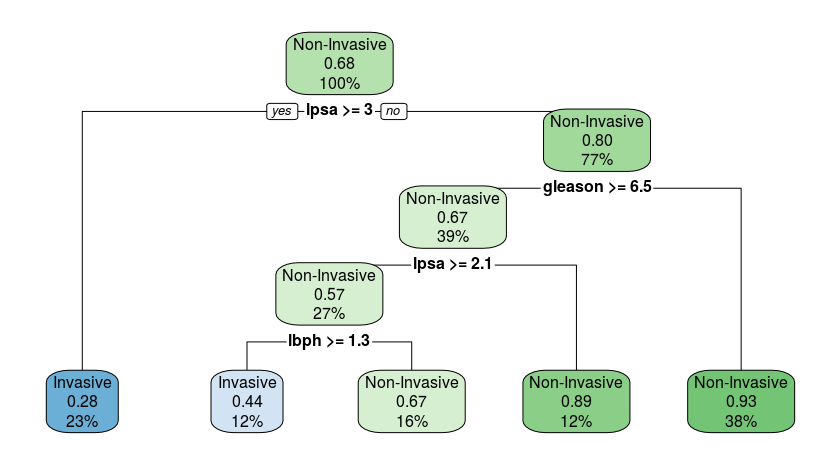
\includegraphics{noninvasive.png}
\end{figure}

And here is the graphical representation of the model. I find that this
version is much easier for me to read than the previous version.


\end{document}
